\tikzstyle{myNode20} = [draw=black, fill=black!20, very thick,
    rectangle, inner sep=5pt, inner ysep=5pt]
\tikzstyle{myNode15} = [draw=black, fill=black!15, very thick,
    rectangle, inner sep=5pt, inner ysep=5pt]
\tikzstyle{myNode10} = [draw=black, fill=black!10, very thick,
    rectangle, inner sep=5pt, inner ysep=5pt]
\tikzstyle{myNode5} = [draw=black, fill=black!5, very thick,
    rectangle, inner sep=5pt, inner ysep=5pt]
\tikzstyle{myNode0} = [draw=white, fill=white, very thick,
    rectangle, inner sep=5pt, inner ysep=5pt]
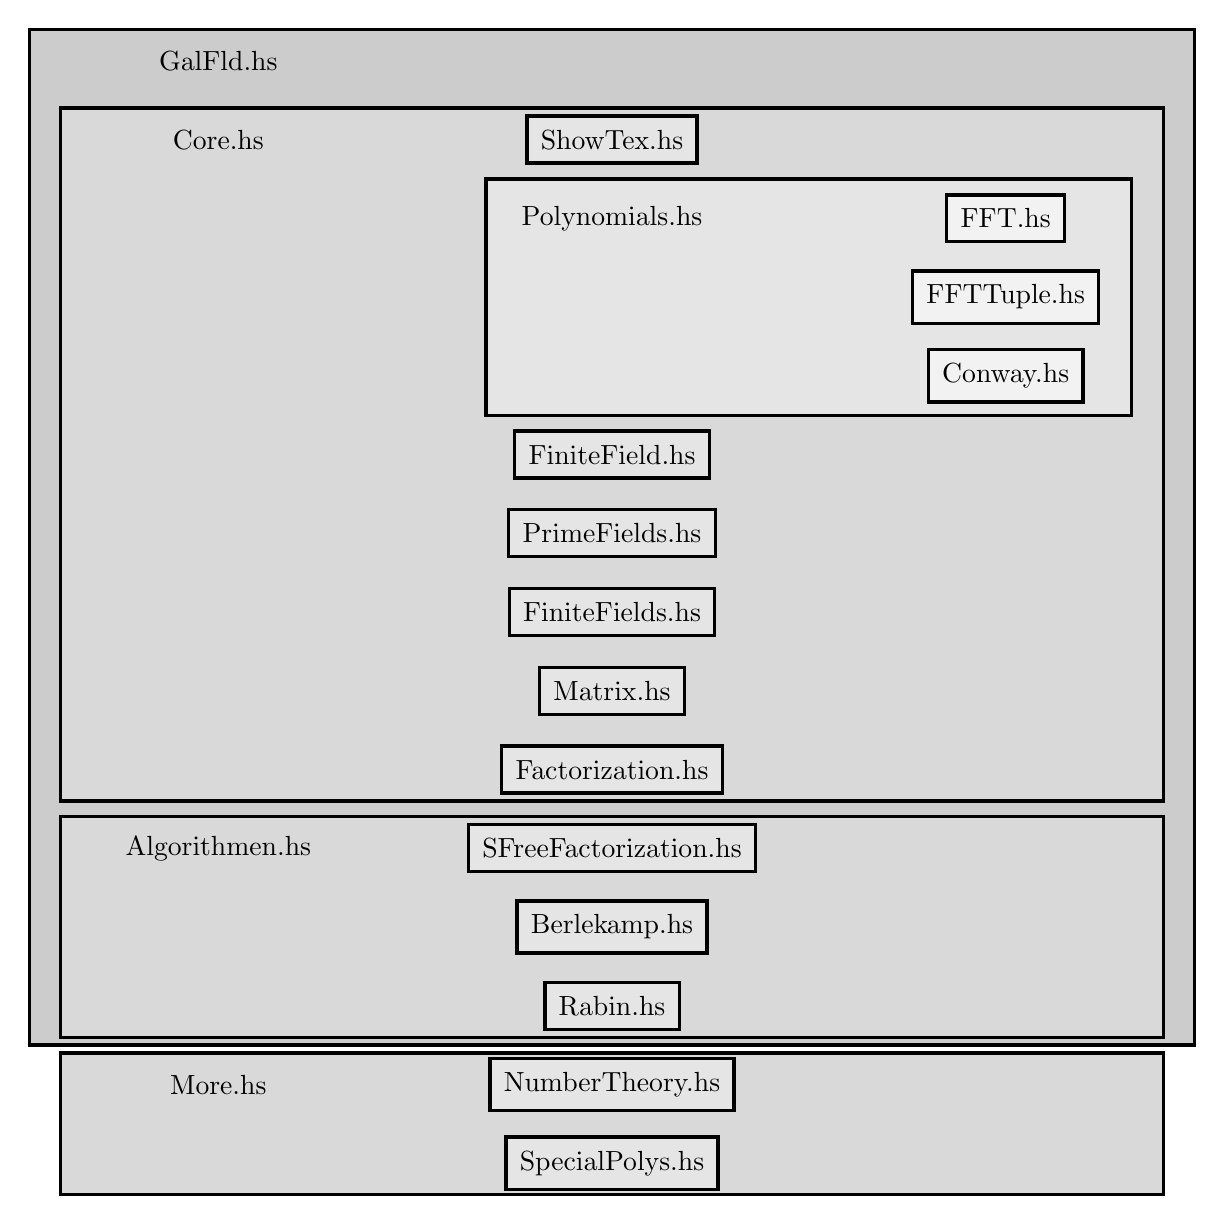
\begin{tikzpicture}

\draw[myNode20] (-2.4,1.4) rectangle (12.4,-11.5);
\draw[myNode15] (-2,0.4) rectangle (12,-8.4);
\draw[myNode15] (-2,-8.6) rectangle (12,-11.4);
\draw[myNode15] (-2,-11.6) rectangle (12,-13.4);
\draw[myNode10] (3.4,-0.5) rectangle (11.6,-3.5);

\node (GalFld) at (0,1) [] {GalFld.hs};
\node (Core) at (0,0) [] {Core.hs};
  \node[myNode10] (ShowTex) at (5,0) [] {ShowTex.hs};
  \node (Polynomials) at (5,-1) [] {Polynomials.hs};
    \node[myNode5] (FFT) at (10,-1) [] {FFT.hs};
    \node[myNode5] (FFTTuple) at (10,-2) [] {FFTTuple.hs};
    \node[myNode5] (Conway) at (10,-3) [] {Conway.hs};
  \node[myNode10] (FiniteField) at (5,-4) [] {FiniteField.hs};
  \node[myNode10] (PrimeFields) at (5,-5) [] {PrimeFields.hs};
  \node[myNode10] (FiniteFields) at (5,-6) [] {FiniteFields.hs};
  \node[myNode10] (Matrix) at (5,-7) [] {Matrix.hs};
  \node[myNode10] (Factorization) at (5,-8) [] {Factorization.hs};
\node (Algorithmen) at (0,-9) [] {Algorithmen.hs};
  \node[myNode10] (SFreeFactorization) at (5,-9) [] {SFreeFactorization.hs};
  \node[myNode10] (Berlekamp) at (5,-10) [] {Berlekamp.hs};
  \node[myNode10] (Rabin) at (5,-11) [] {Rabin.hs};
\node (More) at (0,-12) [] {More.hs};
  \node[myNode10] (NumberTheory) at (5,-12) [] {NumberTheory.hs};
  \node[myNode10] (SpecialPolys) at (5,-13) [] {SpecialPolys.hs};
\end{tikzpicture}
